\documentclass[a4paper,12pt]{article} % тип документа

%  Русский язык
\usepackage[T2A]{fontenc}			% кодировка
\usepackage[utf8]{inputenc}			% кодировка исходного текста
\usepackage[english,russian]{babel}	% локализация и переносы

\usepackage{graphicx, scalerel}               % импорт изображений
\usepackage{wrapfig}                % обтекаемые изображения
\graphicspath{{pictures/}}          % обращение к подкаталогу с изображениями
\usepackage[14pt]{extsizes}         % для того чтобы задать нестандартный 14-ый размер шрифта
\usepackage[warn]{mathtext}         % русский язык в формулах
\usepackage{indentfirst}            % indent first
\usepackage[margin = 25mm]{geometry}% отступы полей
\usepackage[table,xcdraw]{xcolor}   % таблицы
\usepackage{amsmath,amsfonts,amssymb,amsthm,mathtools} % Математика
\usepackage{wasysym}                % ???
\usepackage{upgreek}                % ???  
\usepackage{caption}
\usepackage{multirow}
\captionsetup{labelsep=period}
\usepackage[font=small,labelfont=bf]{caption}
\usepackage{gensymb} % degree symbol
\usepackage{tikz}
\usetikzlibrary{positioning}


\begin{document}
	
	
	\begin{center}
		
		\textbf{НАЦИОНАЛЬНЫЙ ИССЛЕДОВАТЕЛЬСКИЙ УНИВЕРСИТЕТ \\ <<МОСКОВСКИЙ ФИЗИКО-ТЕХНИЧЕСКИЙ ИНСТИТУТ>>}
		\vspace{13ex}
		
		\textbf{Лабораторная работа 5.1.3\\ <<эффект Рамзауэра>>}
		\vspace{40ex}
		
		\normalsize{Шумаков Иван Игоревич \\ студент группы Б01-009\\ 3 курс ФРКТ\\}
	\end{center}
	
	\vfill 
	
	\begin{center}
		г. Долгопрудный\\ 
		2022 г.
	\end{center}
	
	
	\thispagestyle{empty} % выключаем отображение номера для этой страницы
	\newpage

	\textbf{Цель работы:} Исследовать энергетическую зависимоть вероятности рассеяния электронов атомами ксенона.\par
  \textbf{В работе используются:} Тиратрон.\par
    
	\section{Теоретические сведения}
    Рассеяние электрона на атоме можно приближённого рассматривать как рассеяние частицы энергии $E$ на потенциальной яме длины $\ell$ и глубины $U_0$. 
    Уравнение Шрёдингера имеет вид
    \[\Psi'' + k^2 \Psi = 0,\]
    где вне ямы 
    \[k^2 = k_1^2 = \dfrac{2mE}{\hbar^2},\]
    а внутри 
    \[k^2 = k_2^2 = \dfrac{2m(E+U_0)}{\hbar^2}.\]
    Коэффициент прохождения в таком случае равен
    \[D = \dfrac{16 k_1^2 k_2^2}{16k_1^2 k_2^2 + 4(k_1^2 - k_2^2)^2\sin^2(k_2\ell)}.\]
    Заметим, что коэффициент прохождения имеет ряд максимумов и минимумов. 
    Он максимальнем при
    \begin{equation}\label{0}
    \sqrt{\dfrac{2m(E+U_0)}{\hbar^2}}\ell = n\pi,~n=1,2,3,\dots
    \end{equation}
    
    Качественно эффект Рамзауэра можно объяснить, рассмотрев интерференцию прошедшей и дважды отразившейся от оболочки волн де Бройля. 
    Длины волн вне и внутри атома:
    \[\lambda = \dfrac{h}{\sqrt{2mE}},~\lambda_1 = \dfrac{h}{\sqrt{2m(E+U_0)}}.\]
    Соответственно условия на первые интерфереционные максимум и минимум 
    \begin{equation}\label{1}
    2\ell = \dfrac{h}{\sqrt{2m(E_1 + U_0)}},~2\ell = \dfrac{3}{2}\dfrac{h}{\sqrt{2m(E_2 + U_0)}}.
    \end{equation}
    Исключая из этих соотношений глубину ямы, получим
    \begin{equation}\label{2}
    \ell = \dfrac{h\sqrt{5}}{\sqrt{32m(E_2 - E_1)}}.
    \end{equation}
    Глубина ямы при этом равна
    \begin{equation}\label{4}
    U_0 = \dfrac{4}{5}E_2 - \dfrac{9}{5}E_1.
    \end{equation}
  
  \section{Описание установки}
    \begin{figure}[h]
      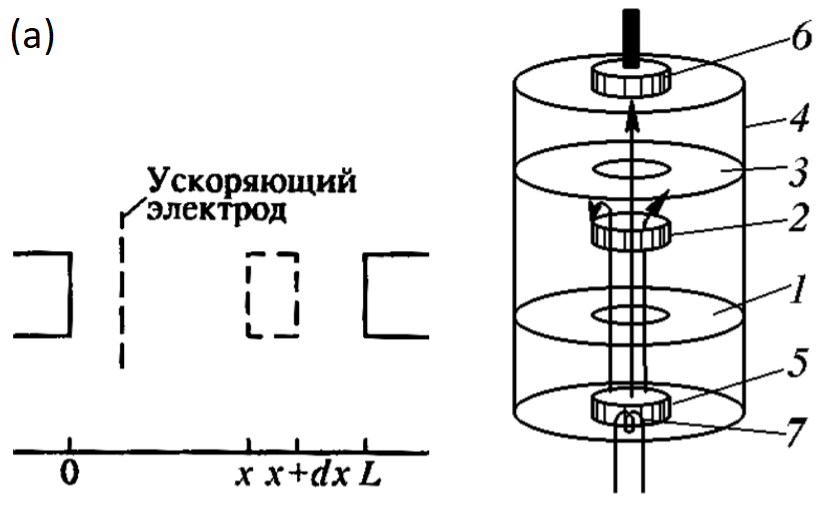
\includegraphics[width=0.42\textwidth]{img/2.png}
      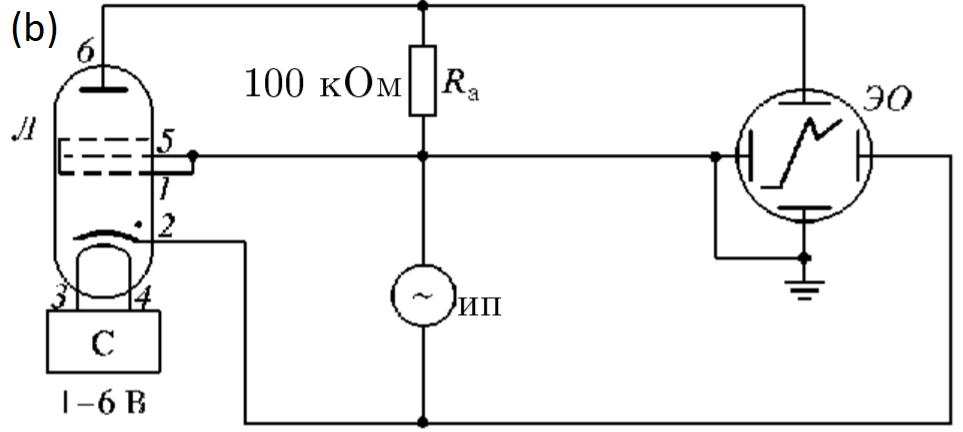
\includegraphics[width=0.58\textwidth]{img/3.png}
      \centering
      \caption{(a) Схема тиратрона (слева) и его конструкция (справа): 1,2,3 -- сетки, 4 -- внешний металлический цилиндр, 5 -- катод, 6 -- анод, 7 -- накаливаемая спираль. (b) Схема включения тиратрона.}
    \end{figure}
    Для изучения эффекта испульзуется тиратрон ТГ3-01/1.3Б, заполненный инертным газом (Рис. 1а). 
    Электроны эмитируются катодом, ускоряются напряжением $V$ и рассеиваются на атомах газа. 
    Сетки соединены между собой и имеют один потенциал, примерно равный потенциалу анода. 
    Рассеянные электроны отклоняются и уходят на сетку, а оставшиеся достигают анода, создавая ток $I_\text{a}$. 
    Таким образом, поток электронов на расстоянии $x$ от ускоряющей сетки уменьшается с ростом $x$. ВАХ анода должна быть
    \begin{equation}\label{3}
      I_\text{a} = I_0 \exp\left( - C w(V) \right),
    \end{equation}
    где $I_0 = eN_0$ -- ток катода, $I_\text{a} = eN_a$ -- ток анода, $C = Ln_\text{a} \Delta_\text{a}$($L$ --  расстояние между катодом и анодом, $\Delta_\text{a}$ -- площадь поперечного сечения атома, $n_\text{a}$ -- концентрация газа в лампе), $w(V)$ -- вероятность рассеяния на атоме.
    Формулу \eqref{3} можно переписать в виде
    \[\tag{5a}\label{5a}
    w(V) = -\dfrac{1}{C}\ln \dfrac{I_\text{a}(V)}{I_0}.
    \]
    \begin{figure}[h]
      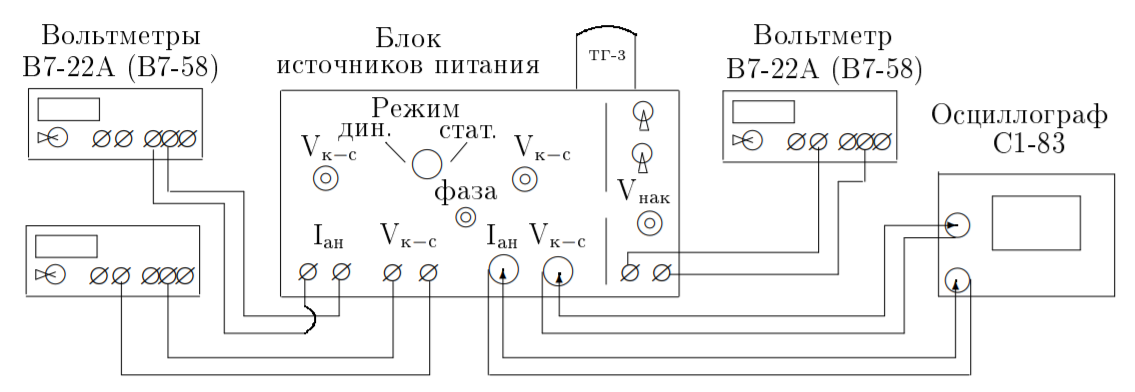
\includegraphics[scale=0.6]{img/1.png}
      \centering
      \caption{Схема установки.}
    \end{figure}\\
    Схема экспериментальной установки, изображанная на Рис. 1b, в нашей работе конструктивно осуществлена следующим образом (Рис. 2): лампа-тиратрон расположена непосредственно на корпусе блока источников питания (БИП), напряжение к электродам лампы подаётся от источников питания, находящихся в корпусе прибора. 
    Регулировка напряжения и выбор режима работы установки производится при помощи ручек управления, выведенных на лицевую панель БИП.

  \section{Ход работы}
    В данной работе были имерены вольт-амперные характеристики инертного газа.
    Они были получены динамическим и статическим метоадами.\par
    Динамическим методом были измерены максимум и минимум тока через инертный газ.
    \begin{table}[h]
      \centering
      \begin{tabular}{|c|c|c|}
      \hline
      \textbackslash{}       & $V_1 = 2.6 [B]$ & $V_2 = 2. 98 [B]$ \\ \hline
      $E_{max} [B]$              & 2       & 2         \\ \hline
      $E_{min} [B]$              & 7.2     & 7.2       \\ \hline
      \end{tabular}
    \end{table}\par
    $V_1 , V_2$ - задерживающее напряжение.
    Погрешность измерения динамического метода равна $\Delta = 0.1 [B]$.
    Расчитаем глубину и ширину ямы:
    \begin{center}
      $l = (3.00 \pm 0.06)$ \AA \\
      $U_0 = (2.16 \pm 0.04)$ эВ \\
    \end{center}
    Далее вольт-амперная характеристика была измерена статическим методом:
  \newpage
    \begin{table}[h!]
      \centering
      \begin{tabular}{|c|c|c|c|c|c|}
      \hline
      $V_1 $ & $U_I$ & E     & $V_2 $ & $U_I$ & E    \\ \hline
             & 0.07  & 0.035 &        & 0.11  & 0.36 \\ \hline
             & 0.09  & 0.199 &        & 0.58  & 0.61 \\ \hline
             & 0.10  & 0.257 &        & 7.96  & 0.32 \\ \hline
             & 0.13  & 0.296 &        & 15.3  & 0.91 \\ \hline
             & 0.37  & 0.421 &        & 34.5  & 1.01 \\ \hline
             & 1.78  & 0.560 &        & 80.2  & 1.17 \\ \hline
             & 2.38  & 0.587 &        & 117   & 1.29 \\ \hline
             & 4.55  & 0.647 &        & 157   & 1.46 \\ \hline
             & 6.25  & 0.676 &        & 178   & 1.61 \\ \hline
             & 9.31  & 0.715 &        & 185   & 1.73 \\ \hline
             & 16.2  & 0.776 &        & 186   & 1.81 \\ \hline
             & 21.4  & 0.811 &        & 173   & 2.08 \\ \hline
             & 24.4  & 0.827 &        & 143   & 2.49 \\ \hline
             & 62.4  & 0.981 &        & 115   & 2.95 \\ \hline
             & 132   & 1.21  &        & 90.3  & 3.50 \\ \hline
             & 172   & 1.38  &        & 75.6  & 3.94 \\ \hline
             & 188   & 1.51  &        & 65.4  & 4.40 \\ \hline
             & 195   & 1.69  &        & 56.2  & 5.00 \\ \hline
             & 190   & 1.85  &        & 52.7  & 5.34 \\ \hline
             & 185   & 1.93  &        & 50.9  & 5.61 \\ \hline
             & 177   & 2.04  &        & 49.8  & 5.85 \\ \hline
             & 155   & 2.35  &        & 48.9  & 5.96 \\ \hline
             & 135   & 2.67  &        & 48.1  & 6.21 \\ \hline
             & 126   & 2.87  &        & 47.8  & 6.42 \\ \hline
             & 101   & 3.62  &        & 48.1  & 6.66 \\ \hline
             & 94.1  & 3.97  &        & 50.4  & 7.86 \\ \hline
             & 89.1  & 4.31  &        & 54.8  & 8.54 \\ \hline
             & 84.9  & 4.71  &        & 63.6  & 9.51 \\ \hline
             & 81.8  & 5.23  &        & 85.1  & 10.6 \\ \hline
             & 81.2  & 5.54  &        & 107   & 11.4 \\ \hline
             & 81.3  & 5.76  &        &       &      \\ \hline
             & 81.7  & 5.92  &        &       &      \\ \hline
             & 82.4  & 6.13  &        &       &      \\ \hline
             & 84.5  & 6.51  &        &       &      \\ \hline
             & 88.9  & 7.03  &        &       &      \\ \hline
             & 97.7  & 7.68  &        &       &      \\ \hline
             & 112   & 8.41  &        &       &      \\ \hline
             & 135   & 9.25  &        &       &      \\ \hline
      \end{tabular}
    \end{table}
  \newpage
    Ток через газ выражается в напряжении на резисторе $R = 10 [kA]$.\par
    По полученным данным были построены графики ВАХ:\par
    \begin{figure}[h]
      \centering
      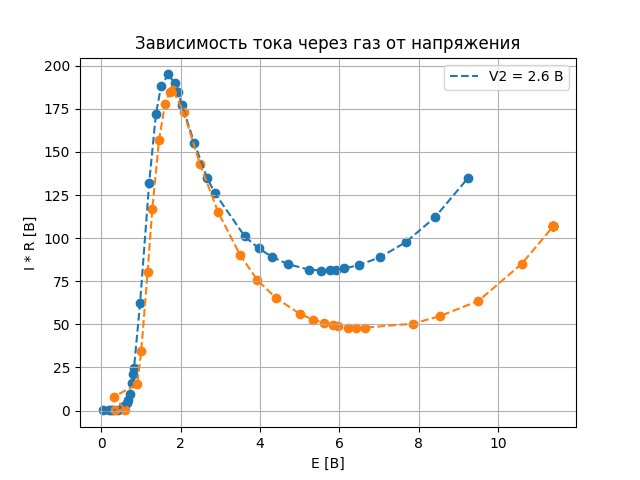
\includegraphics[width=1.2\textwidth]{img/Gra.png}
      \caption{Статический метод}
    \end{figure} 
    По графикам были определены координаты максимумов и минимумов.
    В данном эксперименте только максимумы совпали в пределах погрешности:\par
    \begin{table}[h!]
      \centering
      \begin{tabular}{|c|c|c|c|}
      \hline
      \textbackslash{} & V    & $U_{min}$     & $U_{max}$       \\ \hline
      1                & 2.98 & $5.5 \pm 0.3$ & $1.6 \pm 0.1$ \\ \hline
      2                & 2.60 & $6.4 \pm 0.3$ & $1.8 \pm 0.1$ \\ \hline
      \end{tabular}
    \end{table}
    При измерении минимумов погрешности выше, поскольку они более пологии. 
    Оценка погрешностей производилась по расстоянию до ближайших к экстремумам значений.
  \newpage
    По этим данным были расчитаны параметры ямы:
    \begin{center}
      Для $V_1 = 2.98$ В \\ $l = (3.5 \pm 0.2)$ \AA, $U_0 = (1.4 \pm 0.1)$ эВ \\[0.5 cm]
      Для $V_2 = 2.60$ В \\ $l = (3.2 \pm 0.2)$ \AA, $U_0 = (1.9 \pm 0.1)$ эВ \\[0.5 cm]
    \end{center}  
    Также был построен график зависимоти вероятности рассеяния от напряжения.
    Значение вероятности взято как логарифм тока выраженного в напряжении на резисторе.
    \begin{figure}[h]
      \centering
      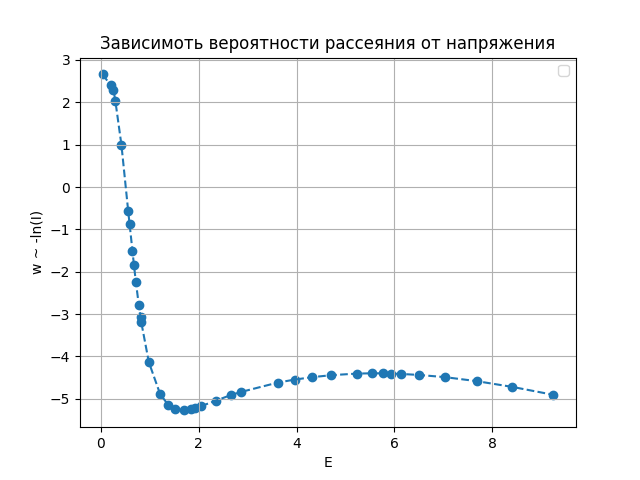
\includegraphics[width=1.2\textwidth]{img/Prob.png}
      \caption{Зависимость вероятности от напряжения}
    \end{figure}\par
    Найдем, при каком значении ускоряющего потенциала на вольт амперной характиристике мы увидили бы максимумы более высоких
    порядков (начиная со второго и так далее). Воспользуемся для этого формулой на дифрационный максимум
    \begin{equation}
        2 l = n \frac{h}{\sqrt{2m (E - U_0)}}
    \end{equation}
    из нее получаем
    \begin{equation}
        U \sim E = \frac{n^2 h^2}{8 l^2 m} - U_0
    \end{equation}
    Для расчета возмем значения $l$ и $U_0$ для напряжения $V_2 = 2.60$ В, поскольку при этом напряжении величина $l$ наиболее
    близка к табличной. Результаты расчетов представлены в таблице.
    \begin{table}[h]
      \centering
      \begin{tabular}{|c|c|}
      \hline
      $n$ & $U$, В     \\ \hline
      1   & 1.81       \\ \hline
      2   & 12.89      \\ \hline
      3   & 31.36      \\ \hline
      4   & 57.22      \\ \hline
      \end{tabular}
    \end{table}
  \section{Вывод}

    В данной работе был подтвержден эффект Рамзауэрас помощью тиратрона.
    По полученным данным были расчитаны характеристики потенциальной ямы атома. 
    Во всех экспериментах были получены схожие значения.
    С учетом погрешности значение ширины ямы примерно равно $l = 3$ \AA, что сходится с реальным значением $l = 280$ пм.
    Разница обусловлена грубостью модели, используемой для расчетов потенциальной ямы.
\end{document}